\documentclass[a4paper,11.5pt]{article}
\usepackage[textwidth=170mm, textheight=230mm, inner=20mm, top=20mm, bottom=30mm]{geometry}
\usepackage[normalem]{ulem}
\usepackage[utf8]{inputenc}
\usepackage[T1]{fontenc}
\PassOptionsToPackage{defaults=hu-min}{magyar.ldf}
\usepackage[magyar]{babel}
\usepackage{amsmath, amsthm,amssymb,paralist,array, ellipsis, graphicx,float}
%\usepackage{marvosym}

\makeatletter
\renewcommand*{\mathellipsis}{%
	\mathinner{%
		\kern\ellipsisbeforegap%
		{\ldotp}\kern\ellipsisgap%
		{\ldotp}\kern\ellipsisgap%
		{\ldotp}\kern\ellipsisaftergap%
	}%
}
\renewcommand*{\dotsb@}{%
	\mathinner{%
		\kern\ellipsisbeforegap%
		{\cdotp}\kern\ellipsisgap%
		{\cdotp}\kern\ellipsisgap%
		{\cdotp}\kern\ellipsisaftergap%
	}%
}
\renewcommand*{\@cdots}{%
	\mathinner{%
		\kern\ellipsisbeforegap%
		{\cdotp}\kern\ellipsisgap%
		{\cdotp}\kern\ellipsisgap%
		{\cdotp}\kern\ellipsisaftergap%
	}%
}
\renewcommand*{\ellipsis@default}{%
	\ellipsis@before
	\kern\ellipsisbeforegap
	.\kern\ellipsisgap
	.\kern\ellipsisgap
	.\kern\ellipsisgap
	\ellipsis@after\relax}
\renewcommand*{\ellipsis@centered}{%
	\ellipsis@before
	\kern\ellipsisbeforegap
	.\kern\ellipsisgap
	.\kern\ellipsisgap
	.\kern\ellipsisaftergap
	\ellipsis@after\relax}
\AtBeginDocument{%
	\DeclareRobustCommand*{\dots}{%
		\ifmmode\@xp\mdots@\else\@xp\textellipsis\fi}}
\def\ellipsisgap{.1em}
\def\ellipsisbeforegap{.05em}
\def\ellipsisaftergap{.05em}
\makeatother

\usepackage{hyperref}
\hypersetup{
	colorlinks = true	
}

\begin{document}
	%%%%%%%%%%%RÖVIDÍTÉSEK%%%%%%%%%%
	\setlength\parindent{0pt}
	\def\s{\hspace{0.2mm}\vphantom{\beta}}
	\def\Z{\mathbb{Z}}
	\def\Q{\mathbb{Q}}
	\def\R{\mathbb{R}}
	\def\C{\mathbb{C}}
	\def\N{\mathbb{N}}
	\def\Ra{\overline{\mathbb{R}}}
	
	\def\sume{\displaystyle\sum_{n=1}^{+\infty}}
	\def\sumn{\displaystyle\sum_{n=0}^{+\infty}}
	
	\def\narrow{\underset{n\rightarrow+\infty}{\longrightarrow}}
	\def\limn{\displaystyle\lim_{n\to +\infty}}
	\def\limx{\displaystyle\lim_{x\to +\infty}}
	
	\theoremstyle{definition}
	\newtheorem{theorem}{Tétel}[subsection] 
	
	\theoremstyle{definition}
	\newtheorem{definition}[theorem]{Definíció} 
	\newtheorem{example}[theorem]{Példa} 
	\newtheorem{task}[theorem]{Feladat} 
	\newtheorem{note}[theorem]{Megjegyzés}
	\newtheorem{revision}[theorem]{Emlékeztető}
	%%%%%%%%%%%%%%%%%%%%%%%%%%%%%%%%%%%%%%%%%%%%%%%%%%%%%%%%%%%%%%%%%%%%%
	\begin{center}
		{\LARGE\textbf{Analízis II.}}
		
		{\Large Előadás jegyzet}
		
		2. óra.
	\end{center}
	A jegyzetet \textsc{Umann} Kristóf készítette Dr. \textsc{Szili} László  előadásán. (\today)
	
	Külön köszönet jár \textsc{Csonka} Szilviának a képek elkészítésért, és \textsc{Solymosi} Zsófiának a jegyzet javításáért.
	\bigskip
	
	Tantárgyi honlap: \url{http://numanal.inf.elte.hu/~szili/Oktatas/An2_BSc_2016/index_An2_2016.htm}
	
	\section{Folytatás.}
	\begin{revision}
		$[a,b]$-n folytonos függvények tulajdonságai.
	\end{revision}
	\begin{theorem}
		(Bolzano)
		
		Tegyük fel, hogy $f:[a,b]\to\R$, továbbá
		
		\[\left.\begin{gathered}
			\text{folytonos } [a,b]\text{-n}\\
			f(a)\cdot f(b)<0\\
		\end{gathered}\right\}\quad \Rightarrow\quad \exists\xi\in[a,b]:\quad f(\xi)=0. \]
		\text{(a két végpontban különböző előjellel)}
		\begin{note}
			$f(a)\cdot f(b) < 0$ azt jelenti hogy különöző pontokban a fv különöző értékeket vesz fel.
		\end{note}
		Szemléletesen:
		
		\begin{figure}[!h]
			\centering
			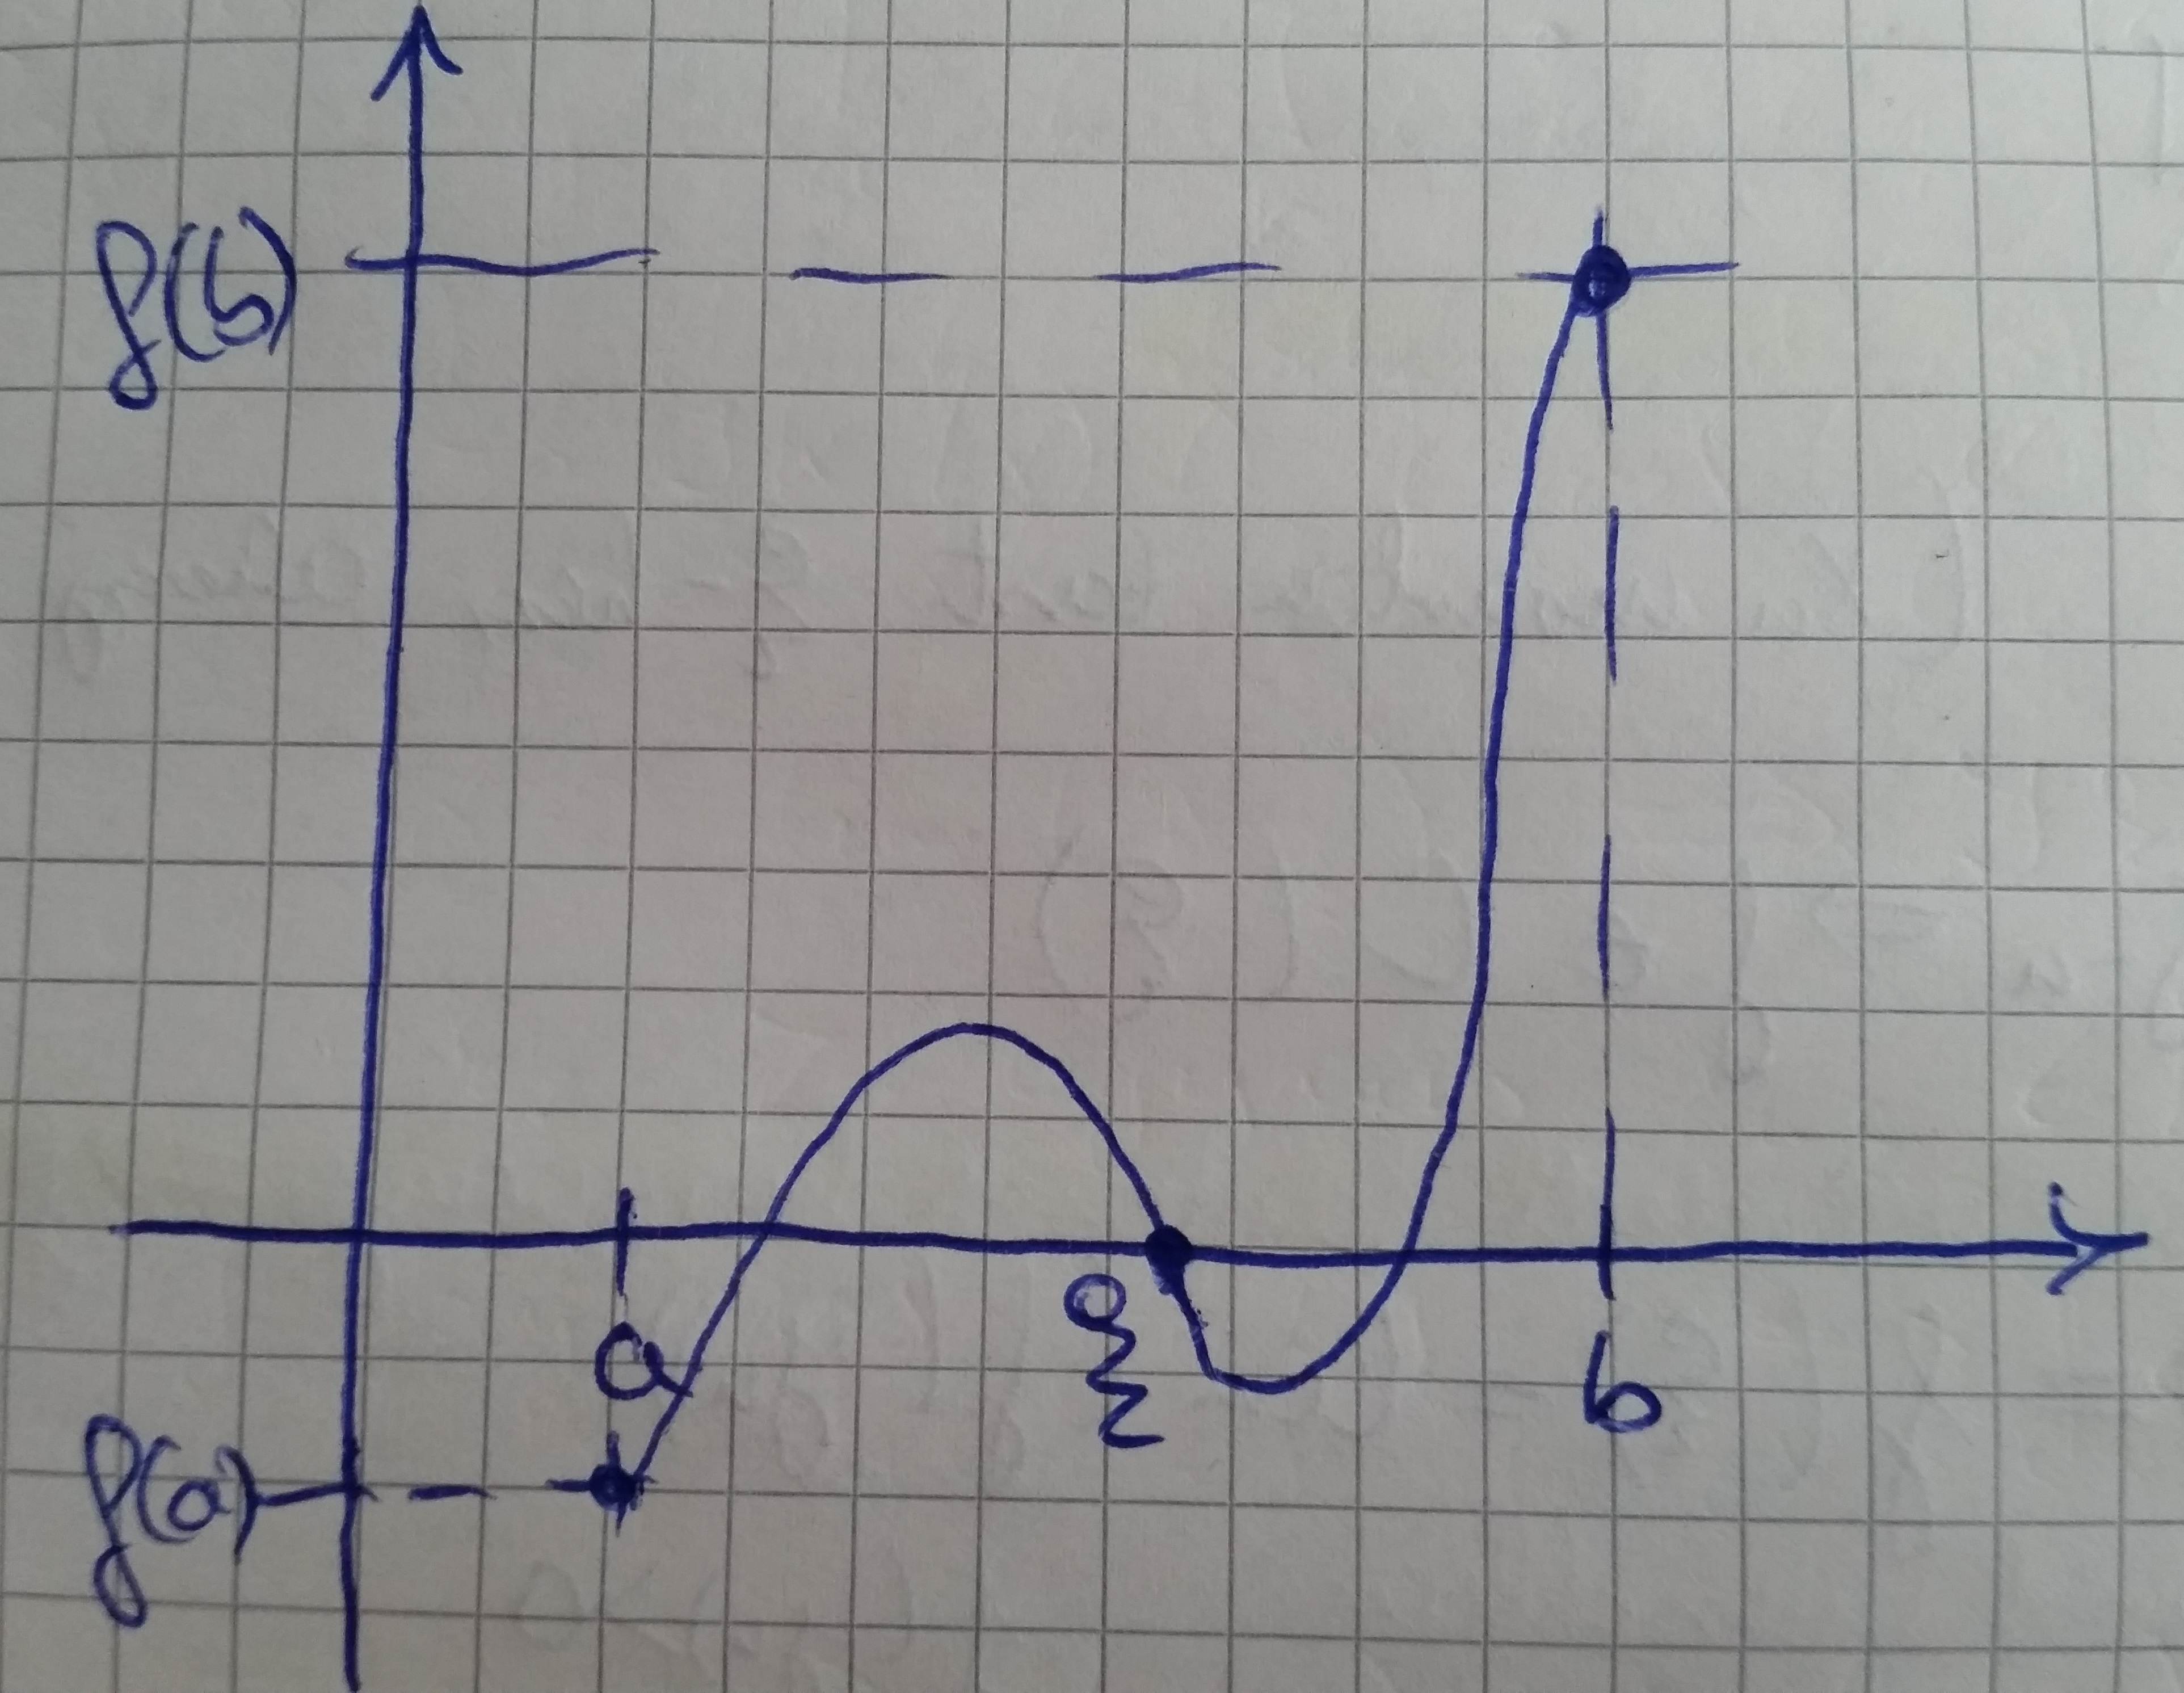
\includegraphics[height=3cm]{kepek/bolzano_theorem.jpg}
			\caption{}\label{fig_bolzano}
		\end{figure}
		\textit{Bizonyítás:} (Bolzano-féle felezési eljárás)
		
		Tegyük fel, hogy $f(a)<0,\quad  f(b)>0.$ \quad Legyen $[x_0, y_0]:=[a,b]$.
		
		\medskip
		Felezzük meg az intervallumot! Legyen $z_0:=\frac{a+b}{2}$. 3 eset lehetséges:
		\begin{enumerate}
			\item $f(z_0)=0 \checkmark$
			\item $f(z_0)>0$ esetén $[x_1,y_1]:=[a,z_0]$.
			\item $f(z_0)<0$ esetén $[x_1,y_1]:=[z_0,b].$
		\end{enumerate}
		Megfelezzük $[x_1,y_1]$-et. Itt is 3 eset lehetséges. (\ldots) Folytatjuk az eljárást.
		
		\medskip
		Az eljárás közben vagy találunk véges sok lépésben olyan  $\xi$-t melyre $f(\xi)=0$, vagy nem. Amennyiben nem,
		$\exists[x_n,y_n]\quad (n\in\N) \quad \text{intervallumsorozat, melyre teljesül hogy}$
		\begin{enumerate}
			\item $[x_{n+1}, y_{n+1}]\subset[x_n,y_n]\quad (\forall n\in\N)$
			\item $f(x_n)<0,\quad f(y_n)>0\quad (\forall n\in\N)$
			\item $y_n-x_n=\displaystyle \frac{b-a}{2^n}$
		\end{enumerate}
		Cantor-féle közösrész tételből következik hogy ezeket az intervallumoknak van közös pontja ha $n\in\N$, azaz:
		\[ \overset{\text{Cantor}}{\underset{\text{tétel}}{\Longrightarrow}}\quad \exists\xi\in\bigcap_{n\in\N}[x_n,y_n],\quad x_n\nearrow\xi, \quad y_n\searrow\xi. \quad (\text{monoton tartanak $\xi$-hez})\]
		$f$ folytonos $[a,b]$-n\quad $\Rightarrow$ \quad $f\in C\{\xi \} \quad \overset{\text{átviteli}}{\underset{\text{elv}}{\Longrightarrow}}\quad \lim(f(x_n))=f(\xi)=\lim(f(y_n))$
		Ha
		\begin{enumerate}
			\item $f(x_n)< 0\quad \Rightarrow\quad \lim(f(x_n))\leq0$
			\item $f(y_n)>0\quad \Rightarrow\quad \lim(f(x_n))\geq 0$
		\end{enumerate}
		Tehát:
		\[\underbrace{f(\xi)\leq 0 \quad \text{és}\quad f(\xi)\geq0}_{\substack{\big\Downarrow\\\displaystyle f(\xi)=0}}\]
		Ezzel a tételt bebizonyítottuk. \quad $\blacksquare$
	\end{theorem}
	\begin{note}
		A tétellel az $f(x)$ egyenlet közelítő megoldását lehet előállítani.
	\end{note}
	\begin{theorem}
		(Bolzano-Darboux)
		
		Ha 
		
		\[\left.\begin{gathered}
		f:[a,b]\rightarrow\R\\
		\text{folyt. } [a,b]\text{-n}
		\end{gathered}\right\}\quad \Rightarrow\quad f \text{ minden } f(a)\text{ és }f(b) \text{ közötti értékeket felvesz.}\]
		\begin{note}
			Ez azt jelenti: ha (pl.) $f(a)<f(b)$,
			\[ \forall c\in(f(a),f(b)) \quad \text{ponthoz}\quad \exists\xi\in[a,b],\quad f(\xi)=c. \]
		\end{note}
		\textit{Bizonyítás:}
		
		A \[\varphi(x):=f(x)-c\quad (x\in[a,b])\] fv.-re alkalmazzuk a Bolzano-tételt.
	\end{theorem}
	\begin{definition}
		Legyen $I\subset\R$ tetszőleges intervallum. Az $f: I\to\R$ fv. \textit{Darboux-tulajdonságú $I$-n}, ha $\forall a, b \in I, \quad a<b$ esetén az $f$ minden $f(a)$ és $f(b)$ közötti értéket felvesz.
	\end{definition}
	\begin{theorem}
		$I\subset\R$ tetszőleges intervallum és $f:I\to\R $ folytonos az $I$-n, $ \Rightarrow f$ Darboux tulajdonságú $I$-n.
		\medskip
		
		\textit{biz nélkül.}
		\begin{note}
			Létezik Darboux tulajdonságú nem folytonos függvény.
		\end{note}
	\end{theorem}
	\begin{theorem}
		(intervallum folytonos képe intervallum.)
		
		$I\subset \R$ tetszőleges intervallum, $f:I\to\R$ folytonos függvény $I$-n. Ekkor $\mathcal{R}_f$ is intervallum.
		\medskip
		
		\textit{biz nélkül.}
	\end{theorem}
	\subsection{Az inverz folytonossága.}
	\begin{revision}
			
		Függvény tulajdonsága, inverze:
		
		\begin{figure}[H]
			\centering
			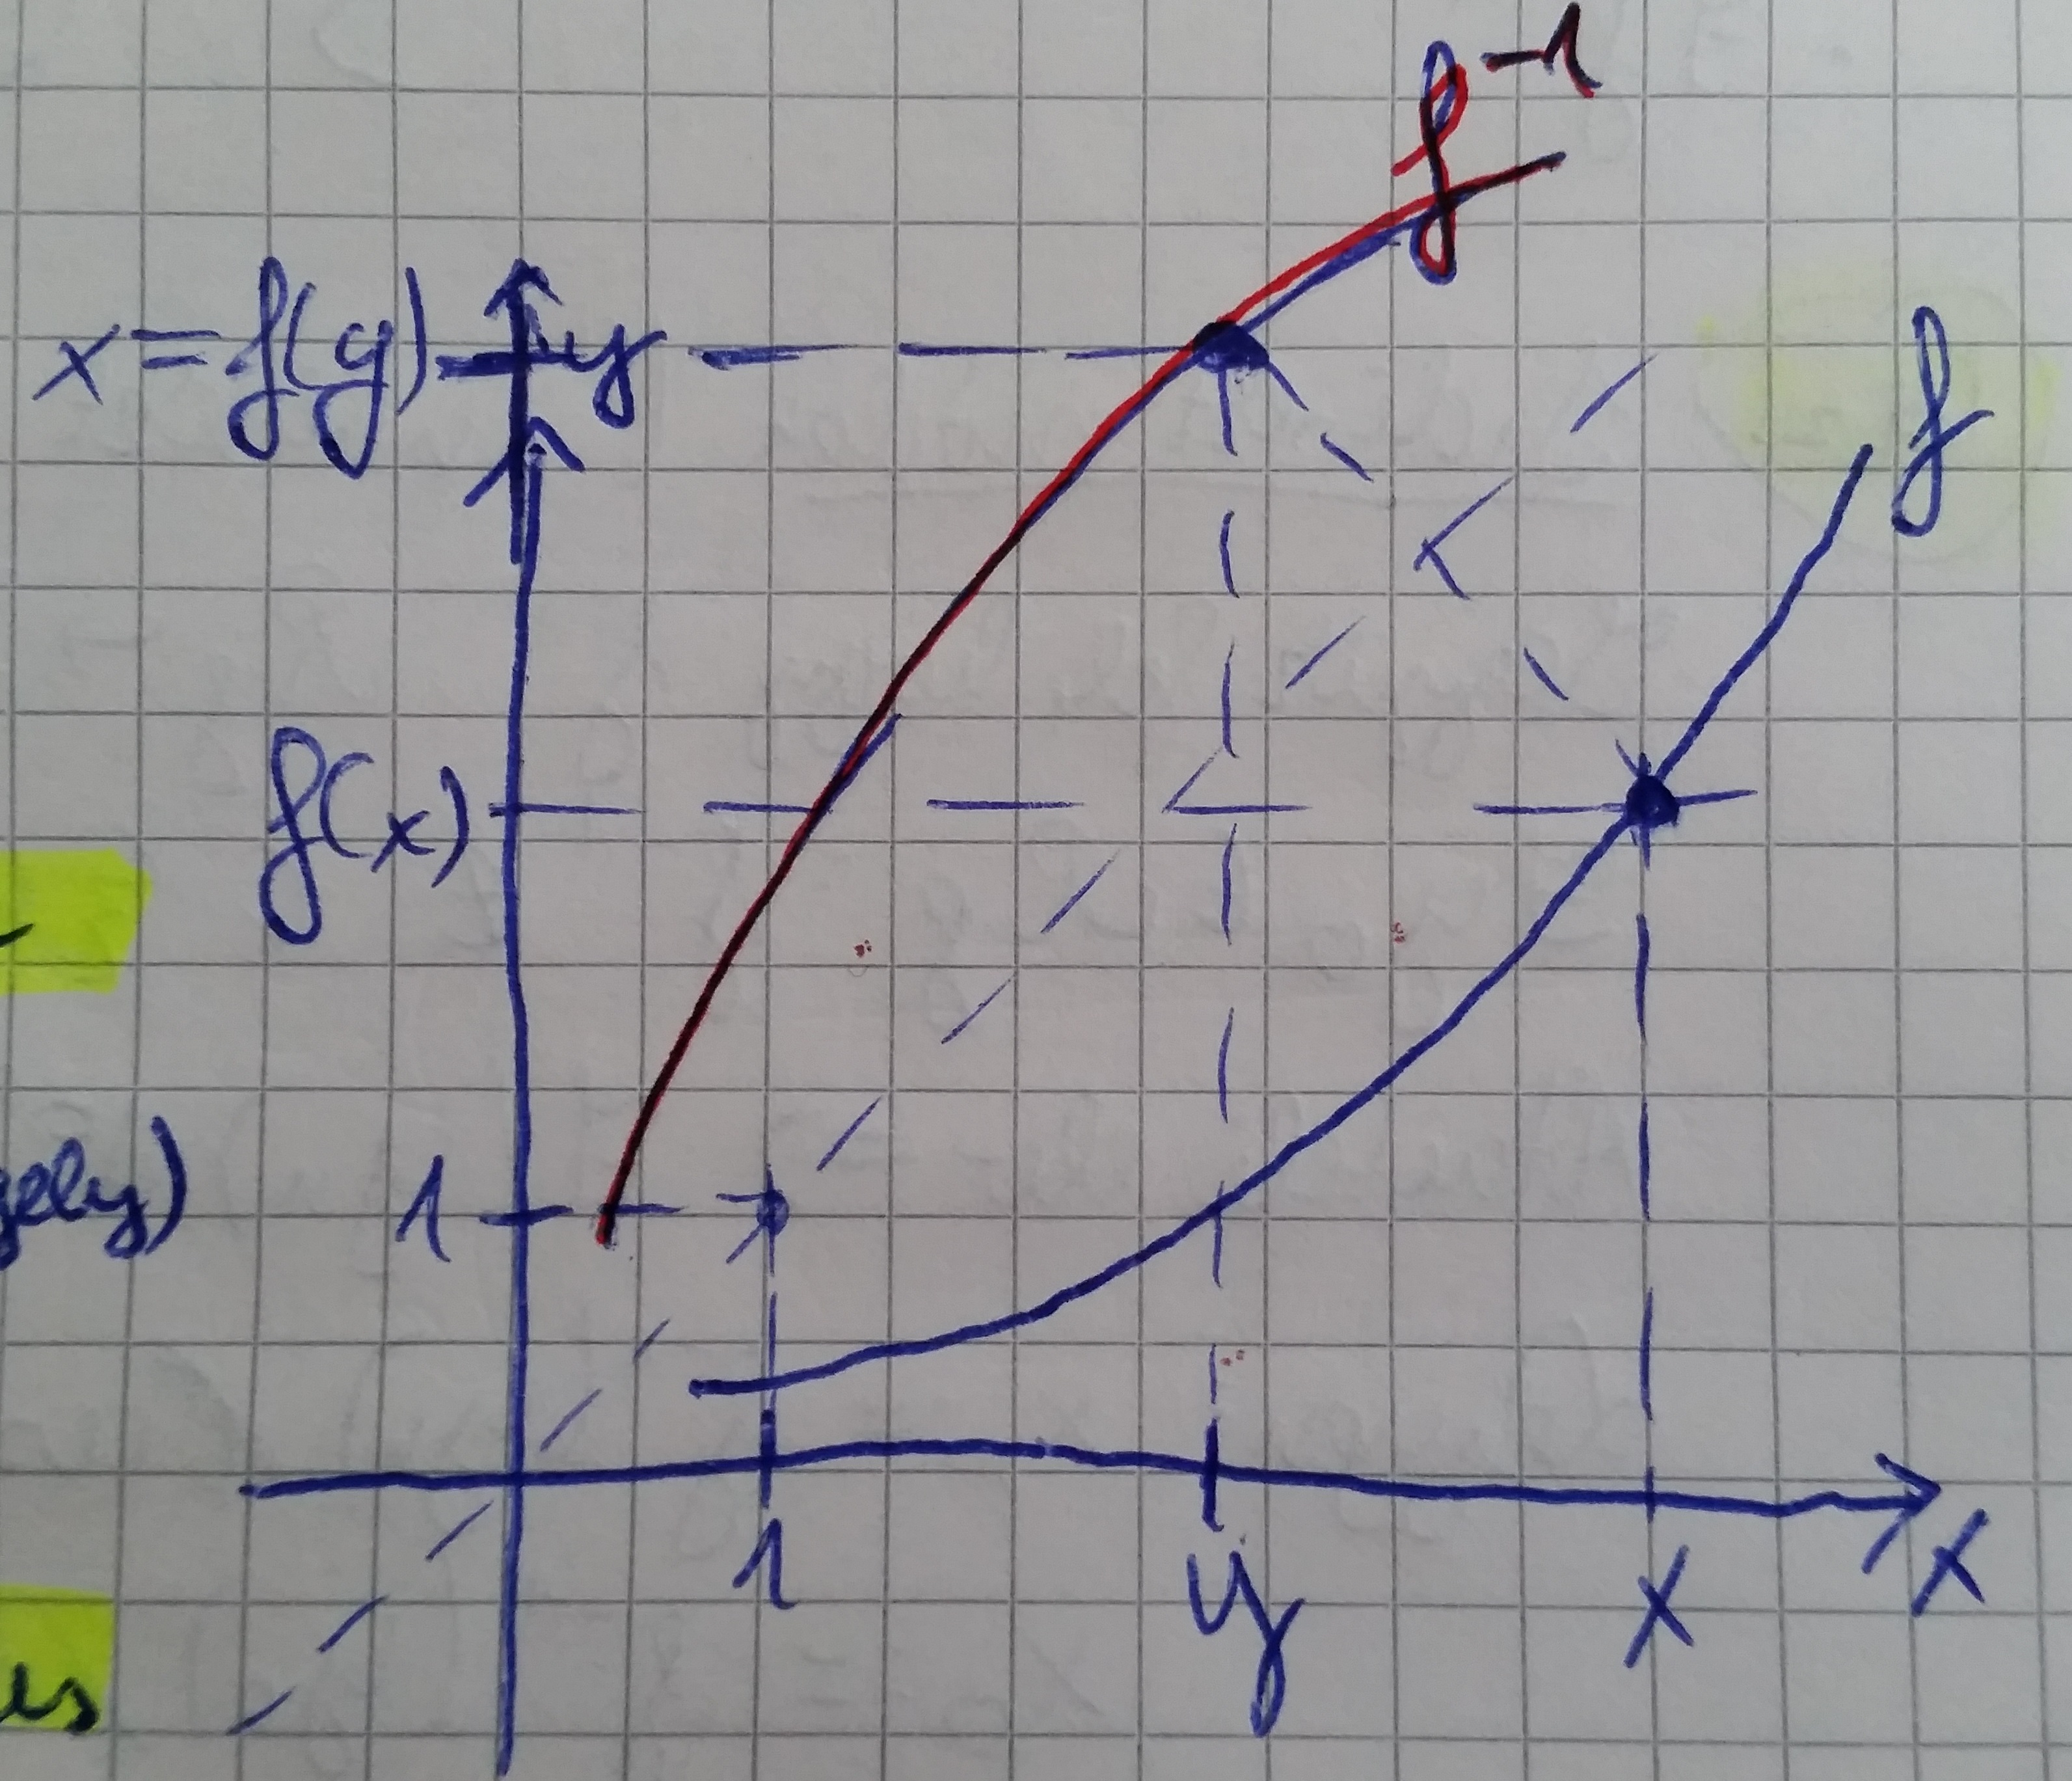
\includegraphics[height=3cm]{kepek/inverse_function.jpg}
			\caption{$f$ és $f^{-1}$ képe az $y=x$ egyenesre szimmetrikus.}\label{fig_emlekezteto_inverz}
		\end{figure}
		\begin{note}
			$f$ folytonossága nem ,,öröklődik'' $f^{-1}$-re.
		\end{note}
	\end{revision}
	\begin{example}\
		
		\begin{figure}[H]
			\centering
			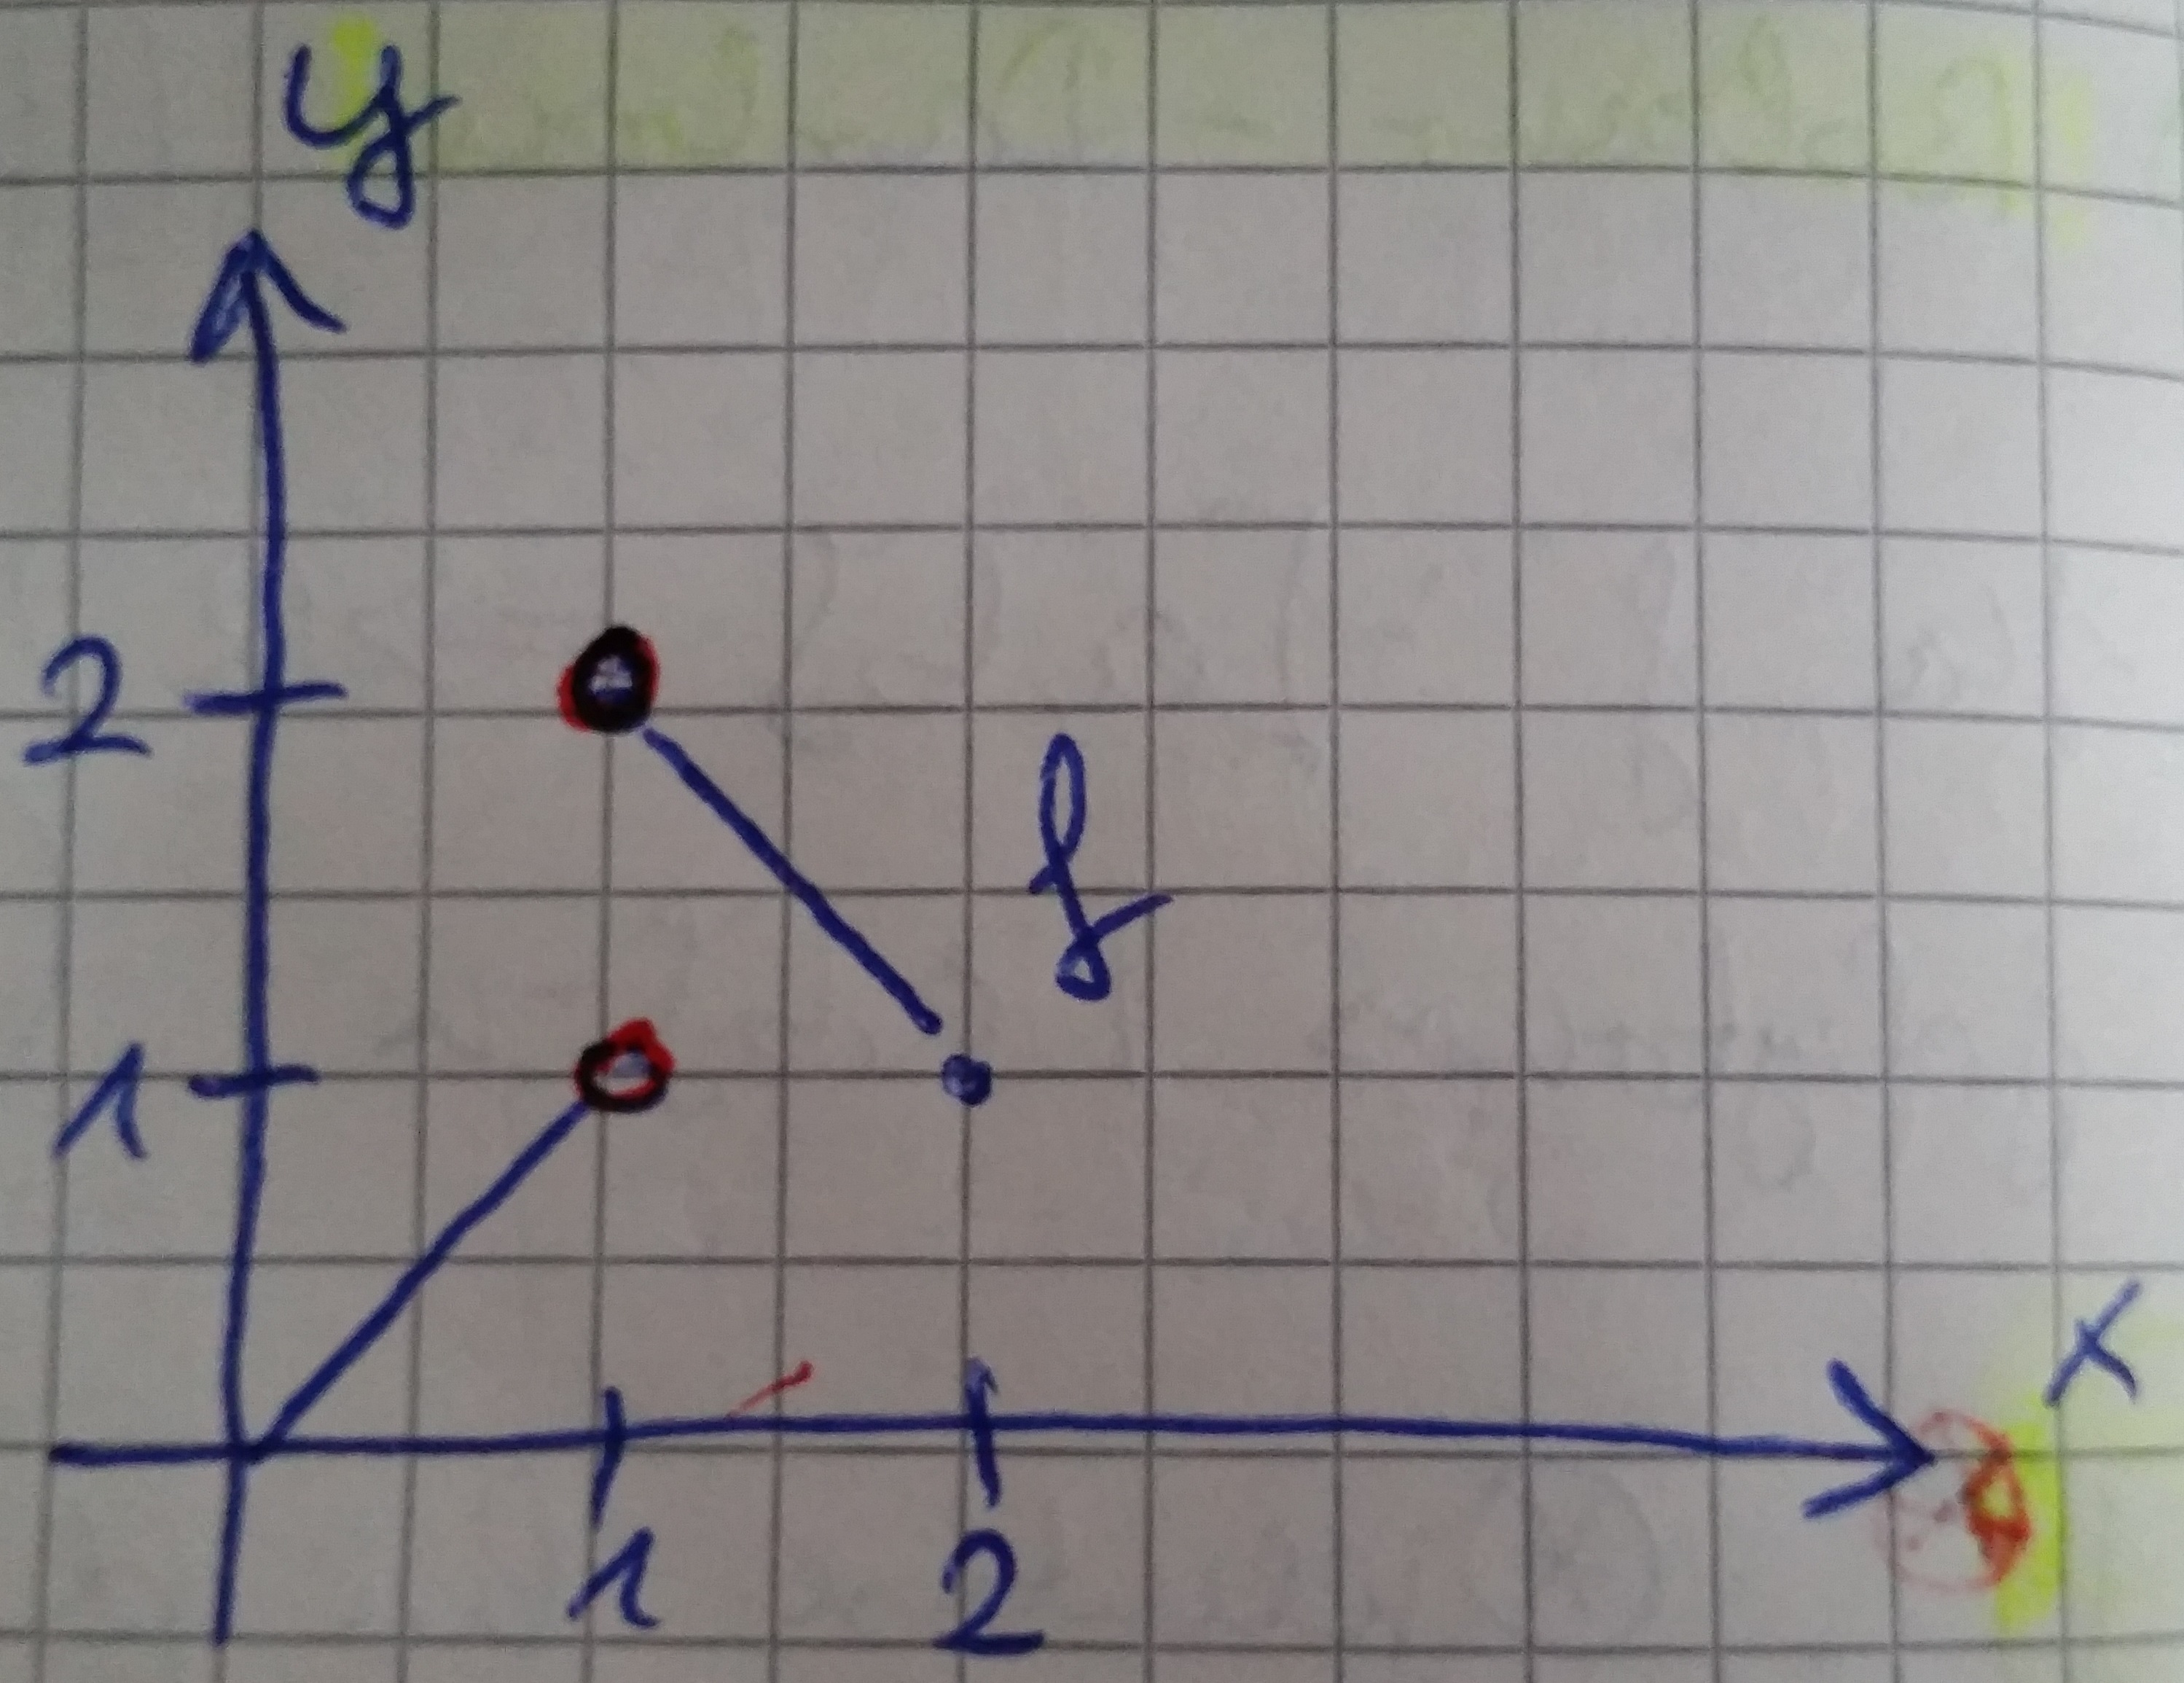
\includegraphics[height=3cm]{kepek/inverse_function_example_1.jpg}\quad \quad \quad 
			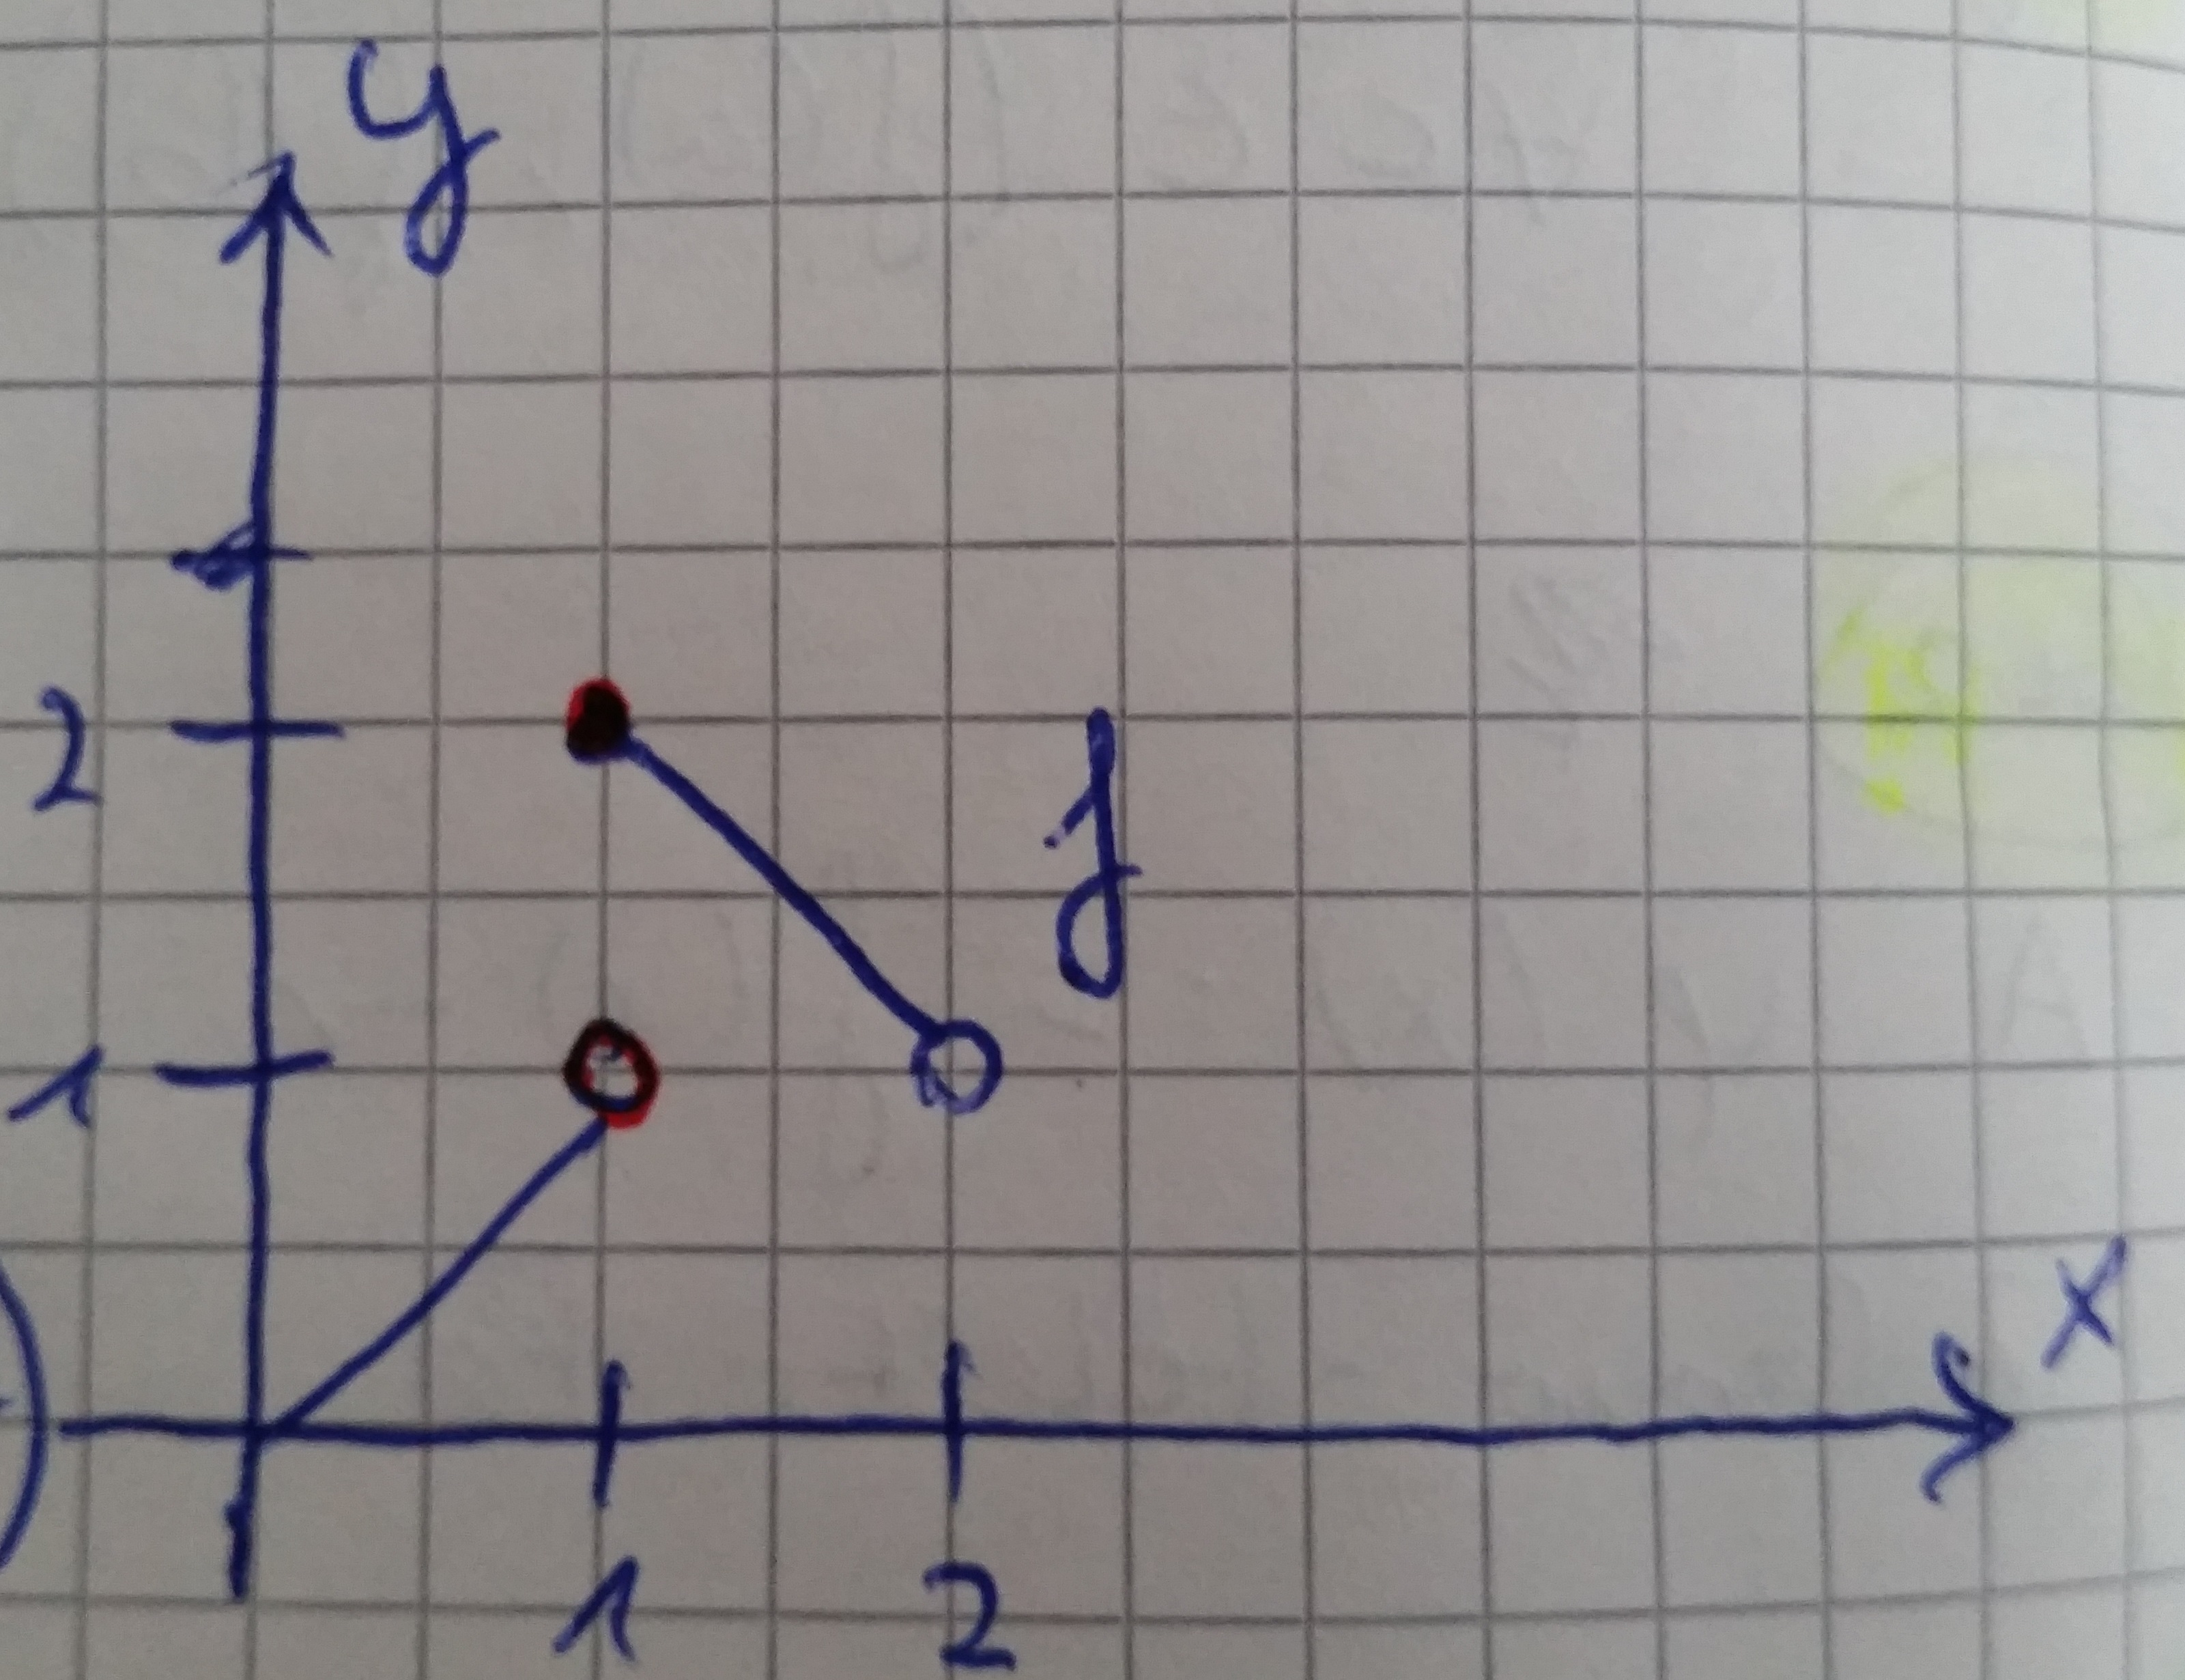
\includegraphics[height=3cm]{kepek/inverse_function_example_2.jpg}
			
			\medskip
			$f(x):=\left\{\begin{gathered}
			x,\quad 0\leq x<1\\
			3-x\quad 1<x\leq 2
			\end{gathered}\right.$
			\quad \quad \quad $f^{-1}(x):=\left\{\begin{gathered}
			x,\quad 0\leq x<1\\
			3-x,\quad 1\leq x<2
			\end{gathered}\right. $
			\caption{}\label{fig_folytonossag_nem_oroklodik}
		\end{figure}
		
		Ekkor:
		\begin{itemize}[$\bullet$]
			\item $f$ folytonos:\quad $\mathcal{D}_f=[0,2)\backslash\{1\}$
			\item $\exists f^{-1};\quad \mathcal{D}_{f^{-1}}=[0,2]$
			\item $f^{-1}\notin C\{1\}$
		\end{itemize}
		Azonban: \quad Ha $\mathcal{D}_f$ egy $[a,b]$-n értelmezett korlátos és zárt intervallum, és $f$ folytonos függvény\quad $\Rightarrow\quad f^{-1}$ is folytonos.
	\end{example}
	\begin{theorem}
		
		Tegyük fel, hogy $f:[a,b]\to\R$,
		\[\left.\begin{gathered}
		\text{folytonos } [a,b]\text{-n}\\
		\exists f^{-1}
		\end{gathered}\right\}\quad \Rightarrow\quad \text{ az }f^{-1}\text{ függvény folytonos }\mathcal{D}_{f^{-1}}=\mathcal{R}_f\text{-en.}\]
		
		\textit{Bizonyítás:} Indirekt, tegyük fel hogy $f^{-1}: \mathcal{R}_f\to[a,b]$ nem folytonos, azaz
		\[ \exists y_0\in\mathcal{R}_f,:\quad f^{-1}\notin C\{y_0\}. \]
		$\text{Átviteli elv}\quad \Rightarrow\quad \exists(y_n)\subset\mathcal{R}_f\quad  \lim(y_n)=y_0,\quad \text{DE}\quad \limn f^{-1}(y_n)\not= f^{-1}(y_0).$
		
		Legyen \[x_n:=f^{-1}(y_n),\quad \text{ azaz}\quad  f(x_n)=y_n \quad \forall n\in\N,\]
		\[ x_0:=f^{-1}(y_0),\quad \text{azaz }\quad f(x_0)=y_0\quad \forall n\in\N.\]
		
		Így: \begin{gather}
			\displaystyle \lim(x_n)\not=x_0.\label{second_lecture_reference}
		\end{gather} Ez azt jelenti, hogy:
		\[ \exists\delta>0:\quad \{ n\in\N\ |\ x_n-x_0\geq \delta \}\quad \text{végtelen halmaz.} \]
		
		Az $(x_n)\subset[a,b]$ korlátos sorozat$\quad \overset{\text{Bolz-Weier}}{\underset{\text{tétel}}{\Longrightarrow}}\quad \exists (x_{\nu_n})$ konvergens részsorozata.
		
		Legyen\quad  $\overline{x}:=\lim(x_{\nu_n})\in[a,b].$ (indirekt módon lehetett bizonyítani)
		
		\[\left.\begin{gathered}
		f\in C\{\overline{x} \}\\
		x_{\nu_n}\to\overline{x}
		\end{gathered}\right\}\quad \overset{\text{átviteli}}{\underset{\text{elv}}{\Longrightarrow}}\quad \underbrace{f(x_{\nu_n})}_{y_{\nu_n}}\longrightarrow f(\overline{x}) \quad (\text{emiatt: }\ref{second_lecture_reference}) \]
		Viszont:
		\[ y_n\to y_0, \quad y_{\nu_n}\to y_0(=f(x_0)) \]
		Ez pedig ellentmondás. \quad $\blacksquare$
	\end{theorem}
	\begin{theorem}
		Tegyük fel, hogy $f:[a,b]\to\R$,
		
		\[\left.\begin{gathered}
		\text{folytonos }[a,b]\text{-n}\\
		\exists f^{-1}
		\end{gathered}\right\}\quad \Rightarrow\quad f\text{ szig. mon. növekvő vagy csökkenő.}\]\\
		
		\textit{biz nélkül.}
	\end{theorem}
	\begin{theorem}
		Legyen $I\subset\R$ tetszőleges intervallum,
		
		\[\left.\begin{gathered}
		f:I\to\R\quad \text{folytonos}\quad I\text{-n}\\
		\exists f^{-1}
		\end{gathered}\right\}\quad \Rightarrow\quad \mathcal{R}_f\text{ is intervallum, és }f^{-1}\text{ folytonos }\mathcal{D}_f\text{-en.}\]
		
		\textit{biz nélkül.}
	\end{theorem}
	\subsection{Szakadási helyek.}
	\begin{definition}
		Legyen $f:\R\to\R,\quad a\in\mathcal{D}_f$ pont \textit{szakadási hely}, ha $f\notin C\{a\}$. 
	\end{definition}
	
	\begin{definition}
		A szakadási helyek osztályozása:
		
		Legyen $f\in\R\to \R, \quad a\in\mathcal{D}_f$
		\begin{enumerate}
			\item $a$ megszüntethető szakadási hely, ha
				\[ \exists\lim_a f \text{\quad véges, és\quad } \lim_a f\not=f(a). \]
				(jobb és bal oldali határértéke is létezik)
			\item $a$ elsőfokú szakadási hely, ha
				\[ \exists \lim_{a+0} f,\quad \exists\lim_{a-0}f \text{\quad végesek, és\quad } \lim_{a+0} f \not= \lim_{a-0}f \] 
			\item Másodfajú szakadási hely az összes többi eset.
		\end{enumerate}
	\end{definition}
\end{document}
